\documentclass[10 pt,usenames,dvipsnames, oneside]{article}
\usepackage{../../../modelo-ensino-medio}



\begin{document}

\begin{center}
  \begin{minipage}[l]{3cm}

\includegraphics[width=2cm]{logo}    
\end{minipage}\hfill
\begin{minipage}[r]{.8\textwidth}
 {\Large \scshape Atividade: Comparação das diferentes categorias na maratona}  
\end{minipage}
\end{center}
\vspace{.2cm}

\ifdefined\prof
%Habilidades da BNCC
\begin{objetivos}
\item \textbf{EM13MAT409} Interpretar e comparar conjuntos de dados estatísticos por meio de diferentes diagramas e gráficos, como o histograma, o de caixa (box-plot), o de ramos e folhas, reconhecendo os mais eficientes para sua análise.
\end{objetivos}

%Caixa do Para o Professor
\begin{goals}
%Objetivos específicos
\begin{enumerate}
\item Comparar distribuições de uma mesma variável para grupos distintos a partir dos histogramas.

\item Perceber a necessidade de usar a mesma escala nos eixos do histograma, para tornar os mesmos comparáveis.
\end{enumerate}

\tcblower

%Orientações e sugestões
Esta atividade introduz os elementos necessários para a comparação de dois histogramas, a saber: mesmas escalas nos eixos e colunas de frequências relativas.

Os histogramas são apresentados com uma série de perguntas de discussão que podem motivar a formulação do conceito de dispersão de forma intuitiva, que será trabalhado na seguinte seção. Além de mostrar como apenas as medidas de posição não dizem suficiente sobre uma distribuição.

As perguntas não têm respostas fechadas, têm o intuito de gerar uma discussão sobre os assuntos já colocados.
\end{goals}

\bigskip
\begin{center}
{\large \scshape Atividade}
\end{center}
\fi

Observe os histogramas da \hyperref[\detokenize{PE104-2:id1}]{figura \ref{\detokenize{PE104-2:id1}}} referentes aos tempos de chegada das categorias “cadeira de rodas”{} e “triciclo de mão”{} na Maratona de Nova Iorque em 2017. Nesse caso, os tempos de chegada foram convertidos para horas e referem-se ao total de participantes que completaram a prova: $51$ na categoria cadeira de rodas e $69$ na categoria triciclo de mão.

\begin{figure}[H]
\centering

\noindent\includegraphics[width=.5\linewidth]{{Histogramas_cadeira_triciclo}.png}
\caption{Histogramas comparativos das quatro modalidades da maratona de Nova Iorque 2017}\label{\detokenize{PE104-2:id1}}\label{\detokenize{PE104-2:id7}}\end{figure}
\begin{enumerate}
\item {} 
Compare as escalas utilizadas na construção destes histogramas, tanto no eixo horizontal, como no eixo vertical. O que você observou?

\item {} 
Em qual categoria se encontra o atleta que completou a maratona no maior tempo?

\item {} 
Você consegue estimar o tempo médio destas categorias observando os histogramas? Você acha que os tempos médios dessas duas categorias serão muito diferentes dos tempos médios das categorias de homens e de mulheres (atividade \hyperref[\detokenize{PE104-2:ativ-maratona-categoria-homens}]{Categoria Homens na Maratona})?

\item {} 
Observe o quadro a seguir e marque as médias (em horas) nos histogramas. Comente sobre a posição da média em cada caso e sobre a simetria ou assimetria de cada distribuição de dados.

\begin{table}[H]
\centering
\caption{Média das quatro categorias da maratona de Nova Iorque 2017}
\begin{tabular}{|c|c|c|}
\hline
\tcolor{Categoria} & \tcolor{Cadeira de rodas} & \tcolor{Triciclo de mão} \\
\hline
Média & 2,59 & 2,73 \\
\hline
\end{tabular}
\end{table}


\item {} 
Observe que as médias não são muito diferentes. Se você conhecesse apenas a média, seria capaz de perceber a forma destes histogramas? Por quê?

\item {} 
Comparando os dois histogramas, qual distribuição apresenta maior dispersão? Por quê?

\item A partir dos esquemas de cinco números para os tempos de chegada nas categorias cadeira de rodas e triciclo de mão, informados a seguir, construa os respectivos boxplots sem sinalização de valores discrepantes, usando a mesma escala de valores para as duas categorias.

\begin{table}[H]
\centering

\begin{tabular}{|*{6}{c|}}
\hline
\tcolor{Categoria} & \tcolor{Mínimo} & \tmat{$Q_1$} & \tmat{$Q_2$} & \tmat{$Q_3$} & \tcolor{Máximo} \\
\hline
Cadeira de rodas & $1{,}62$ & $1{,}8$ & $2{,}09$ & $2{,}68$ & $7{,}{,}81$ \\
\hline
Triciclo de mão & $1{,}48$ & $1{,}78$ & $2{,}38$ & $3{,}09$ & $9{,}52$ \\
\hline
\end{tabular}
\end{table}

\end{enumerate}

\ifdefined\prof
\begin{solucao}

\begin{enumerate}
\item As escalas horizontal e vertical são coincidentes em ambos os histogramas para permitir a comparação. Isto foi discutido no capítulo \hyperref[est1-chap]{\textbf{A Natureza da Estatística}}.
\item Observando-se os histogramas o maior tempo está na categoria de Triciclo de mão.
\item A simples visualização pode remeter a estimativa de 4 horas para estas categorias, valor bem maior do que as médias para homens e mulheres (ativ-maratona-categoria-homens). No entanto, este valor excede muito as médias reais, apresentadas. Isto mostra que estimar o centro de equilíbrio de uma distribuição a partir do histograma não é trivial.
\item Ambos os histogramas apresentam assimetria à direita: grande concentração de dados à esquerda e forma alongada para a direita.
\item Não é possível, a informação apenas da média é insuficiente para caracterizar a forma do histograma. Outras informações são necessárias para isto.
\item O triciclo de mão apresenta maior dispersão, considerando a amplitude.
\item Na figura a seguir veja uma cosntrução dos boxplots sem sinalização dos valores discrepantes.
\begin{figure}[H]
\centering

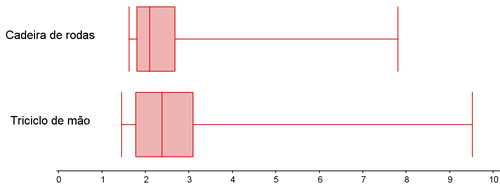
\includegraphics[width=.75\linewidth]{boxplotcadeiratriciclo_svd.png}
\caption{Boxplots sem sinalização de valores discrepantes para os tempos de chegada em horas das categorias “cadeira de rodas”{} e “triciclo de mão”}
\label{}
\end{figure}
\end{enumerate}

\end{solucao}
\fi

\end{document}